% ---------------------------------------------------------------
% Paper A -- Elsevier submission (elsarticle).
%
% Build:  latexmk -pdf elsarticle-main.tex
%
% Requires elsarticle.cls and elsarticle-num.bst, available from
% https://www.elsevier.com/authors/policies-and-guidelines/latex-instructions
% or from any full TeX Live installation (tlmgr install elsarticle).
%
% Class options:
%   preprint         single column, for arXiv and for circulating drafts
%   review           double spaced, wide margins, line numbers -- use this
%                    for the actual submission, as most Elsevier journals
%                    request it
%   5p               final two-column layout, for checking length only
% ---------------------------------------------------------------
\documentclass[preprint,12pt,authoryear]{elsarticle}

\usepackage[T1]{fontenc}
\usepackage[utf8]{inputenc}
\usepackage{amsmath}
\usepackage{amssymb}
\usepackage{booktabs}
\usepackage{multirow}
\usepackage{graphicx}
\usepackage[usenames,dvipsnames]{xcolor}
\usepackage{tikz}
\usetikzlibrary{arrows.meta,positioning,decorations.pathreplacing}
\usepackage{url}

% elsarticle loads natbib itself; \biboptions sets the citation style.
% Numeric citations are used throughout, so that prose naming an author is
% not duplicated by the citation itself.
\biboptions{numbers,sort&compress}

\journal{Future Generation Computer Systems}

\begin{document}

\begin{frontmatter}

\title{What Determines Reported Savings in Carbon-Aware\\
       Virtual Machine Scheduling?\\
       Capacity, Home Region, and Region-Set Composition}

% --- Authors -----------------------------------------------------
% Replace names, affiliations and email addresses. The corresponding
% author is marked with \corref; move the marker if that is not the
% first author.
\author[aff1]{Riman Mandal\corref{cor1}}
\ead{FIRST.AUTHOR@EXAMPLE.EDU}
\cortext[cor1]{Corresponding author.}

\author[aff1]{Second Author}
\ead{SECOND.AUTHOR@EXAMPLE.EDU}

\author[aff2]{Third Author}
\ead{THIRD.AUTHOR@EXAMPLE.EDU}

\author[aff2]{Fourth Author}
\ead{FOURTH.AUTHOR@EXAMPLE.EDU}

\affiliation[aff1]{organization={School of Computer Science and Engineering,
                                 INSTITUTION},
                   city={CITY},
                   postcode={POSTCODE},
                   country={COUNTRY}}

\affiliation[aff2]{organization={DEPARTMENT, INSTITUTION},
                   city={CITY},
                   postcode={POSTCODE},
                   country={COUNTRY}}

% --- Abstract ----------------------------------------------------
\begin{abstract}
Reported reductions from carbon-aware virtual machine scheduling vary widely
across the literature, from a few per cent to more than eighty. We show that
much of this variation is produced not by the schedulers but by three choices in
the evaluation that are seldom reported. Using CloudSim Plus with published
hourly emission factors for seven grid regions and a production virtual machine
trace, and adopting the host platform, simulator and baseline of a recent
spatio-temporal scheduling study, we isolate each in turn. First, the value of
deadline flexibility is conditional on load: widening the deadline margin from
6\,h to 48\,h reduces emissions by $32.1 \pm 6.1$\,\% at 13\,\% capacity
utilisation but by $0.9 \pm 0.6$\,\% at 82\,\%. Second, the performance of a
time-shifting policy is determined by the region in which its workload
originates rather than by the temporal structure it exploits: the correlation
with the origin region's mean carbon intensity is between $+0.941$ and $+0.998$,
while the correlation with its diurnal amplitude is indistinguishable from zero,
and results across seven candidate origins span a factor of 3.6. Third, holding
workload, scheduler and hardware fixed, one region set reports approximately
twice the reduction of another at matched utilisation, because it contains a
region 4.7 times cleaner than its nearest rival. A single mechanism underlies
all three: emissions track the concentration of work into the cleanest reachable
grid, with a correlation below $-0.93$ throughout, and the largest reductions we
observe coincide with placing 95\,\% or more of the workload in one region. The
results hold across five workload samples, two seasons, two workload classes and
two host power models. We conclude with the four quantities an evaluation of
carbon-aware scheduling should report if its figures are to be comparable.
\end{abstract}

% --- Highlights (Elsevier requires 3-5, each under 85 characters) --
\begin{highlights}
\item Deadline flexibility is worth 32\% at low load and under 1\% at high load
\item Time-shifting results are set by the origin region, not by daily variation
\item The same scheduler reports twice the savings on a more degenerate region set
\item Emissions track concentration of work into one grid, with $r$ below $-0.93$
\item Four quantities are proposed that such evaluations should always report
\end{highlights}

\begin{keyword}
carbon-aware scheduling \sep cloud computing \sep virtual machine placement \sep
deadline-constrained scheduling \sep evaluation methodology \sep CloudSim Plus
\end{keyword}

\end{frontmatter}

% ---------------------------------------------------------------
\section{Introduction}
\label{sec:intro}

The carbon intensity of electricity varies by hour and by location. Scheduling
computation to exploit that variation, by deferring work to cleaner hours or by
relocating it to cleaner grids, is now a well-established line of research, and
the reductions reported for it are large. They are also inconsistent. Studies
of temporal shifting report reductions that vary substantially with the region
examined \cite{wiesner2021letswait}, and studies of combined spatial and temporal
shifting report ranges wider still. Zanotto et
al.~\cite{zanotto2025usercentric}, whose formulation this paper takes as its
starting point, report a 79.25\,\% reduction against a carbon-agnostic baseline
in their most permissive configuration and 13.46\,\% in their most restrictive
one. Work examining the limits of these techniques has established that headline
figures depend heavily on the assumptions behind them
\cite{sukprasert2024limitations}, but the parameters responsible have not been
isolated individually.

The two configurations that produce the 13\,\% and the 79\,\% differ in two
respects at once: the permissive one allows fifty simultaneous jobs per region
where the restrictive one allows five, and it draws on a different set of
candidate regions. Neither parameter is varied alone, so the six-fold difference
cannot be attributed to either. The same study is explicit that the per-region
concurrency limit is consequential and that its estimation is left for future
work. This paper takes up that question, and finds that the answer accounts for
much of the range.

This paper argues that a substantial part of the variation is not a property of
the schedulers at all. It is produced by three choices in the evaluation which
are seldom reported, and each of which moves the reported figure by more than
the difference between the policies being compared.

The first is capacity. A scheduler that defers a request to a cleaner hour can
do so only if capacity is free in that hour. Evaluations that place a workload
into an effectively unconstrained pool measure the benefit of flexibility under
the most favourable condition available, and this condition is rarely stated.
We find that widening the deadline margin from 6\,h to 48\,h reduces emissions
by 32.1\,\% when the system runs at 13\,\% utilisation and by 0.9\,\% when it
runs at 82\,\%, a difference of more than thirty-fold produced entirely by how
heavily the system is loaded.

The second is the origin region assigned to a time-shifting policy. Such a
policy holds work in one region and moves it only in time, so its result is
partly a statement about that region. We find that the correlation between the
mean carbon intensity of the origin region and the emissions the policy achieves
is between $+0.941$ and $+0.998$, whereas the correlation with the region's
diurnal amplitude, the quantity the policy actually acts upon, is
indistinguishable from zero. Across the seven candidate origins in our primary
region set, the same policy yields results spanning a factor of 3.6. A single
reported figure is one draw from that spread, and the conventional choice of
origin selects the cleanest available grid.

The third is the composition of the candidate region set. Running an identical
workload and an identical scheduler at matched utilisation over two region sets,
we find that one reports approximately twice the reduction of the other at every
operating point. The set that reports more contains a region 4.7 times cleaner
than its nearest rival, so that a single destination is optimal for nearly every
request; the set that reports less does not.

These are not competing explanations for the spread in the literature but
complementary ones, and they share a mechanism. Across every configuration we
examine, the correlation between the fraction of the workload placed in the
busiest region and total emissions is below $-0.93$. Carbon-aware placement
policies work by concentrating load into the cleanest reachable grid; capacity
governs how much can be concentrated, the origin region governs where a
time-shifting policy starts from, and the region set governs how much is to be
gained by concentrating at all. The reductions these policies report are, to
first approximation, measurements of the concentration they achieve.

The consequence for practice is that the largest reductions are obtained in
precisely the configurations least likely to be deployable. At the lowest
utilisation we examine, the policies achieving the largest reductions place
between 95\,\% and 98\,\% of the workload in a single region.

Our contributions are as follows.

\begin{itemize}
\item We isolate the interaction between capacity utilisation and deadline
      margin, and show that the value of deadline flexibility is conditional on
      load rather than being a property of the workload or the scheduler
      (Section~\ref{sec:res-capacity}).
\item We show that the reported performance of a time-shifting policy is
      determined by its origin region rather than by the temporal structure it
      exploits, and quantify the resulting spread
      (Section~\ref{sec:res-home}).
\item We show that reported savings scale with the degree to which the candidate
      region set contains a dominant clean region, holding workload, scheduler
      and hardware fixed (Section~\ref{sec:res-regionset}).
\item We establish that these results hold across five workload samples, two
      seasons, two workload classes, two region sets and two host power models,
      and we report the accounting basis on which each is measured
      (Section~\ref{sec:res-robustness}).
\end{itemize}

We adopt the host platform, the simulator, the carbon-agnostic baseline, the
per-region concurrency constraint and the deadline-margin levels of Zanotto et
al.~\cite{zanotto2025usercentric}, so that differences between their reported
figures and ours cannot be attributed to any of those. Where we depart from them
is in varying one parameter at a time, in sweeping the origin region of the
time-shifting policy rather than fixing it, and in reporting emissions on an
explicitly stated accounting basis. The evaluation
uses published hourly emission factors \cite{maji2022carboncast} and a
production virtual machine trace \cite{cortez2017resourcecentral}, and each
experimental cell is checked to confirm that every virtual machine executed in
the region its planner selected.

\section{Related work}
\label{sec:related}

\subsection{Temporal shifting}

Deferring flexible work to hours of lower carbon intensity was examined
systematically by Wiesner et al.~\cite{wiesner2021letswait}, who characterised
delay-tolerant workloads and quantified the potential for temporal shifting in
four regions over a year. Their finding that the achievable reduction depends
strongly on the region examined is the starting point for
Section~\ref{sec:res-home}: we ask which property of the region is responsible,
and find that it is the region's mean intensity rather than its temporal
structure. Earlier work on scheduling around on-site renewable supply
\cite{goiri2011greenslot,grange2018greenit} addresses a related problem, though
with generation local to the datacentre rather than grid intensity as the
varying quantity.

\subsection{Spatial and spatio-temporal shifting}

Relocating work between grids has been studied both as load balancing across
geo-distributed datacentres \cite{zhou2013carbonaware} and, more recently, as
carbon-aware placement in production settings
\cite{radovanovic2023carbonaware,souza2023casper}. Sukprasert et
al.~\cite{sukprasert2023spatiotemporal,sukprasert2024limitations} examine the
limits of both temporal and spatial shifting and conclude that reported benefits are sensitive to the
assumptions under which they are measured. Our work is complementary: where they
establish that the assumptions matter in aggregate, we isolate three specific
parameters and quantify each separately, holding the remainder fixed.

Zanotto et al.~\cite{zanotto2025usercentric} evaluate combined spatial and
temporal shifting for non-preemptible virtual machines under a Kubernetes-based
architecture. They formulate placement as a binary integer program solved one
request at a time against a greedily updated occupancy matrix, and evaluate it in
CloudSim Plus against a carbon-agnostic round-robin baseline, with a per-machine
power profile drawn from SPECpower and virtual machine requests sampled from a
production trace. Their formulation is the direct antecedent of the policies
compared in Section~\ref{sec:results}, and we adopt their host platform,
simulator, baseline, per-region concurrency constraint and deadline-margin levels
so that our results and theirs differ in as few respects as possible.

Their constraint limiting each region to $M_j$ simultaneous jobs is introduced
explicitly to prevent what they term the ``black hole'' case, in which the
optimiser assigns the entire workload to the single cleanest region. They
observe that the limit governs the outcome, that a permissive limit concentrates
nearly all work in one region while a restrictive one distributes it, and that
the value of $M_j$ must be determined experimentally. They leave that estimation
as future work. Sections~\ref{sec:res-capacity} and~\ref{sec:res-regionset}
address it, and find that the parameter accounts for a larger share of the
variation in reported savings than the scheduling policy does.

\subsection{Carbon intensity data and its representation}

The choice of carbon intensity signal is itself consequential. Maji et
al.~\cite{maji2024greenmirage} show that location-based and market-based
estimation methods can lead to different conclusions about the efficacy of the
same optimisation. Forecast-based scheduling depends further on prediction
quality, for which day-ahead \cite{maji2022dacf} and multi-day
\cite{maji2022carboncast} methods have been developed. We use published
lifecycle emission factors throughout and plan against ground truth, so that
the parameters under study are not confounded with prediction error; the effect
of forecast quality is a separate question that this paper deliberately does not
address. We note that Zanotto et al.~\cite{zanotto2025usercentric} report
closely comparable results under forecast and under perfect foresight,
which supports treating prediction error as separable from the parameters
studied here.

Infrastructure for carbon-aware experimentation has also received attention.
Testbeds such as Vessim \cite{wiesner2023vessim} and virtualised energy systems
such as Ecovisor \cite{souza2023ecovisor} provide environments in which
carbon-aware applications can be developed and evaluated. Our aim differs: we do
not propose a new environment but examine what an evaluation conducted in such
an environment is measuring.

\subsection{Simulation and power modelling}

CloudSim \cite{calheiros2011cloudsim} and its successor CloudSim Plus
\cite{silvafilho2017cloudsimplus} are widely used for cloud resource-management
studies, and we adopt the latter. Reported energy figures in such studies depend
on the host power model, and Ismail and Materwala \cite{ismail2020serverpower}
survey the models in use and their accuracy. We use a measured
SPECpower\_ssj2008 curve for the specific host modelled
\cite{spec2024xr8620t} and, because the choice is consequential, repeat the
entire evaluation under a linear approximation to establish which of our
conclusions depend on it (Section~\ref{sec:res-robustness}).

\subsection{Position of this work}

Prior work has proposed carbon-aware scheduling policies and has examined their
limits. What has not been established is how much of the variation in reported
savings is attributable to the evaluation configuration rather than to the
policies themselves. This paper addresses that question directly, and the answer
bears on how such evaluations should be reported.

% ---------------------------------------------------------------
% Schematic figures. TikZ only; no external image dependencies.
% ---------------------------------------------------------------

\begin{figure*}[t]
\centering
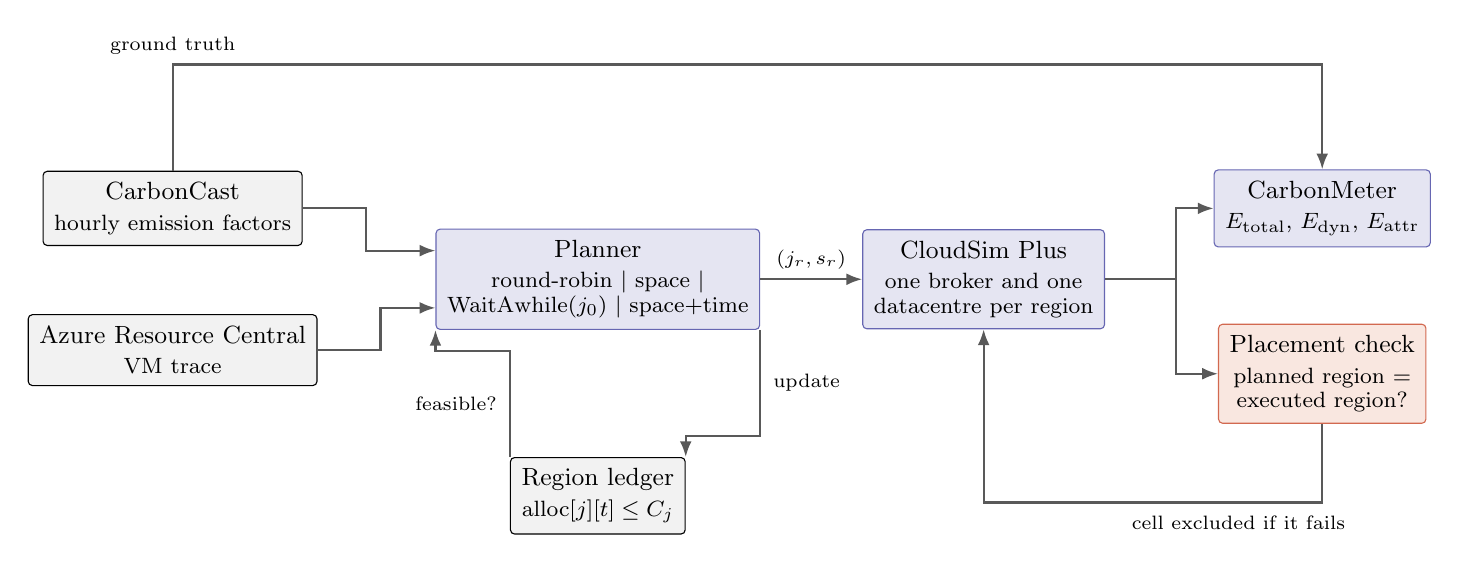
\begin{tikzpicture}[
  font=\small,
  box/.style={draw, rounded corners=1.5pt, align=center, inner sep=4pt,
              minimum height=9mm, font=\small},
  data/.style={box, fill=black!5},
  proc/.style={box, fill=NavyBlue!10, draw=NavyBlue!60},
  check/.style={box, fill=BrickRed!8, draw=BrickRed!60},
  ar/.style={-{Latex[length=2mm]}, thick, draw=black!65},
]

\node[data] (ci)  at (0,1.35)  {CarbonCast\\\footnotesize hourly emission factors};
\node[data] (vm)  at (0,-0.45) {Azure Resource Central\\\footnotesize VM trace};

\node[proc] (plan) at (5.4,0.45)
  {Planner\\\footnotesize round-robin $\mid$ space $\mid$\\[-2pt]
   \footnotesize WaitAwhile($j_0$) $\mid$ space+time};
\node[data] (ledger) at (5.4,-2.3)
  {Region ledger\\\footnotesize $\mathrm{alloc}[j][t] \le C_j$};

\node[proc] (sim) at (10.3,0.45)
  {CloudSim Plus\\\footnotesize one broker and one\\[-2pt]
   \footnotesize datacentre per region};

\node[proc]  (meter) at (14.6,1.35)
  {CarbonMeter\\\footnotesize $E_{\mathrm{total}}$, $E_{\mathrm{dyn}}$,
   $E_{\mathrm{attr}}$};
\node[check] (valid) at (14.6,-0.75)
  {Placement check\\\footnotesize planned region $=$\\[-2pt]
   \footnotesize executed region?};

\draw[ar] (ci.east) -- ++(0.8,0) |- (plan.170);
\draw[ar] (vm.east) -- ++(0.8,0) |- (plan.190);

\draw[ar] (plan.south east) -- ++(0,-1.35)
      node[midway, right=1pt, font=\scriptsize] {update} -| (ledger.north east);
\draw[ar] (ledger.north west) -- ++(0,1.35)
      node[midway, left=1pt, font=\scriptsize] {feasible?} -| (plan.south west);

\draw[ar] (plan.east) -- node[above, font=\scriptsize] {$(j_r, s_r)$} (sim.west);

\draw[ar] (ci.north) |- ++(0,1.35)
      node[above, font=\scriptsize, pos=0.72] {ground truth} -| (meter.north);

\draw[ar] (sim.east) -- ++(0.9,0) |- (meter.west);
\draw[ar] (sim.east) -- ++(0.9,0) |- (valid.west);

\draw[ar] (valid.south) -- ++(0,-1.0)
      node[below left=1pt and -12pt, font=\scriptsize] {cell excluded if it fails}
      -| (sim.south);

\end{tikzpicture}
\caption{Evaluation pipeline. The planner assigns each request a region and a
start hour subject to the per-region concurrency cap, and the resulting schedule
is then executed in the simulator, so that emissions are obtained from simulated
host power rather than from the planner's own objective. Every cell is checked
after execution to confirm that each virtual machine ran in the region its
planner selected; cells that fail are excluded rather than reported. The carbon
trace enters twice, once as the planning signal and once as the measurement
signal, which are identical here and separable when forecast quality is under
study.}
\label{fig:pipeline}
\end{figure*}


\begin{figure}[t]
\centering
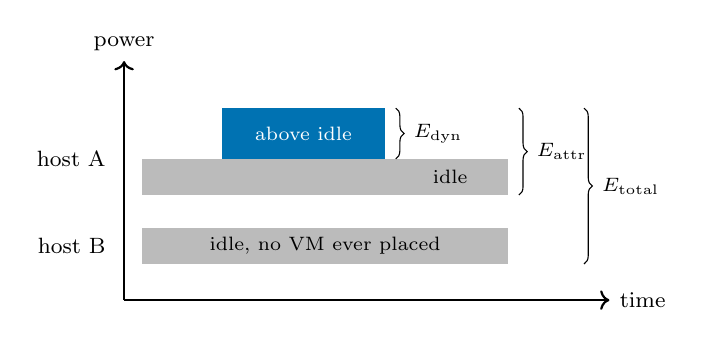
\begin{tikzpicture}[font=\small, scale=0.92]

\definecolor{idlec}{HTML}{BBBBBB}
\definecolor{dync}{HTML}{0072B2}

\draw[->, thick] (0,0) -- (6.7,0) node[right, font=\footnotesize] {time};
\draw[->, thick] (0,0) -- (0,3.3) node[above, font=\footnotesize] {power};

\node[font=\footnotesize, anchor=east] at (-0.12,1.95) {host A};
\fill[idlec] (0.25,1.45) rectangle (5.3,1.95);
\fill[dync]  (1.35,1.95) rectangle (3.6,2.65);
\node[font=\scriptsize, white] at (2.475,2.30) {above idle};
\node[font=\scriptsize] at (4.5,1.70) {idle};

\node[font=\footnotesize, anchor=east] at (-0.12,0.75) {host B};
\fill[idlec] (0.25,0.5) rectangle (5.3,1.0);
\node[font=\scriptsize] at (2.775,0.75) {idle, no VM ever placed};

\draw[decorate, decoration={brace, amplitude=3pt}]
  (3.75,2.65) -- (3.75,1.95)
  node[midway, right=3pt, font=\scriptsize] {$E_{\mathrm{dyn}}$};
\draw[decorate, decoration={brace, amplitude=3pt}]
  (5.45,2.65) -- (5.45,1.45)
  node[midway, right=3pt, font=\scriptsize] {$E_{\mathrm{attr}}$};
\draw[decorate, decoration={brace, amplitude=3pt}]
  (6.35,2.65) -- (6.35,0.5)
  node[midway, right=3pt, font=\scriptsize] {$E_{\mathrm{total}}$};

\end{tikzpicture}
\caption{The three accounting bases, shown schematically for a two-host fleet.
$E_{\mathrm{total}}$ charges every provisioned host for the whole window and is
therefore invariant to placement in a fixed fleet. $E_{\mathrm{dyn}}$ charges
only draw above idle and is unaffected by how many hosts a schedule activates.
$E_{\mathrm{attr}}$ charges the full draw of hosts that carry load and nothing
for hosts that do not, so it responds both to regional placement and to
consolidation. Host~B is provisioned in all three cases; it contributes to
$E_{\mathrm{total}}$ alone.}
\label{fig:bases}
\end{figure}

% ---------------------------------------------------------------
% Paper A -- Sections 3 and 4
% Requires: booktabs, amsmath, siunitx (optional), url
% ---------------------------------------------------------------

\section{Method}
\label{sec:method}

\subsection{Overview}

We evaluate carbon-aware placement of non-preemptible virtual machines across
geographically distributed datacentres. A workload of independent VM requests
arrives over a 720\,h horizon. Each request must be assigned to one region and
one start hour, subject to a per-region concurrency cap and a per-request
deadline. Once started, a VM runs to completion in the region where it was
placed; migration and preemption are outside the scope of this study, following
the assumptions of Zanotto et al.~\cite{zanotto2025usercentric}.

The evaluation is implemented on CloudSim Plus 8.5.7~\cite{silvafilho2017cloudsimplus}
under Java~17. Placement
decisions are taken by a planner operating on an occupancy ledger, and the
resulting schedule is then executed in the simulator so that host-level power
draw, and hence emissions, are obtained from simulated execution rather than
from the planner's own cost model. This separation matters: the planner
minimises a carbon-intensity objective, whereas the reported emissions depend
additionally on how many physical hosts the schedule activates. Sections
\ref{sec:accounting} and \ref{sec:validity} describe the accounting and the
checks that connect the two.

\subsection{System model}

Let $J$ denote the set of eligible regions and $T = \{0,\dots,H-1\}$ the hours
of the horizon, with $H = 720$. Each request $r$ is a tuple
$(p_r, m_r, d_r, a_r, \delta_r)$ giving its core count, memory, duration in
hours, arrival hour and deadline hour. A placement assigns $r$ to a region
$j_r \in J$ and a start hour $s_r \ge a_r$. The request meets its deadline when
$s_r + d_r \le \delta_r$.

Regional capacity is expressed as an occupancy matrix
$\mathrm{alloc}[j][t]$ counting VMs running in region $j$ at hour $t$, subject
to
%
\begin{equation}
\mathrm{alloc}[j][t] \;\le\; C_j
\qquad \forall j \in J,\; \forall t \in T ,
\label{eq:cap}
\end{equation}
%
where $C_j$ is the per-region concurrency cap. Constraint~\eqref{eq:cap}
represents the finite capacity a tenant can command in any single region and is
the parameter whose effect this paper isolates.

Each region hosts one datacentre containing an identical fleet of homogeneous
hosts. The host is a Dell PowerEdge XR8620T with an Intel Xeon Gold 6433N
(32 cores at 2.00\,GHz) and 256\,GB of memory. This is the platform modelled by
Zanotto et al.~\cite{zanotto2025usercentric}, who likewise draw its power profile from SPECpower and likewise
evaluate on CloudSim Plus against a carbon-agnostic round-robin baseline;
adopting the same host removes hardware as a source of difference between their
reported figures and ours. Each core is modelled as a processing element of
2000\,MIPS.
A VM requests $p_r$ processing elements and $m_r$ memory, and executes a single
cloudlet of length $2000 \cdot d_r \cdot 3600$ MI at full CPU utilisation, so
that its runtime equals $d_r$ hours.

\subsection{Host power model}
\label{sec:power}

Host power is taken from the published SPECpower\_ssj2008 result for the same
machine \cite{spec2024xr8620t} (Dell Inc., PowerEdge XR8620T with Xeon Gold 6433N,
tested 15 July 2024, 6\,564 overall ssj\_ops/watt). The sensitivity of simulated
energy figures to the power model adopted is well documented
\cite{ismail2020serverpower}. Because the simulated host matches the
benchmarked one in core count, clock and memory, the measured curve is used
without rescaling. Table~\ref{tab:power} reports it.

\begin{table}[t]
\centering
\caption{Measured host power at decile load points (SPECpower\_ssj2008).}
\label{tab:power}
\begin{tabular}{lrrrrrrrrrrr}
\toprule
Load (\%) & 0 & 10 & 20 & 30 & 40 & 50 & 60 & 70 & 80 & 90 & 100 \\
Power (W) & 230 & 244 & 260 & 273 & 301 & 340 & 372 & 385 & 400 & 416 & 420 \\
\bottomrule
\end{tabular}
\end{table}

Power at intermediate utilisations is obtained by linear interpolation between
adjacent measured points, since SPEC publishes no finer resolution. Two
properties of this curve affect the results. First, the machine draws 230\,W at
idle against a 420\,W peak, an idle fraction of 55\,\%; the range a scheduler
can influence is therefore 190\,W per host. Second, the curve is not linear: it
is nearly flat between 0\,\% and 30\,\% load, rises steeply between 30\,\% and
60\,\%, and flattens again above 70\,\%. A linear model fitted only to the idle
and peak points misprices both ends of the range traversed by the capacity
sweep. Section~\ref{sec:robustness-design} describes how sensitivity to this
choice is tested.

\subsection{Carbon accounting}
\label{sec:accounting}

Emissions are obtained by integrating host power against regional carbon
intensity. Sampling occurs on every simulation clock tick, with a datacentre
scheduling interval of 300\,s, and each interval is charged at the carbon
intensity of the hour in which it begins. For a host $h$ in region $j$ with
utilisation $u_h(t)$, the instantaneous rate is
$P(u_h(t)) \cdot \mathrm{CI}_j(t)$, where $P$ is the interpolated curve of
Table~\ref{tab:power} and $\mathrm{CI}_j(t)$ the regional carbon intensity in
gCO\textsubscript{2}eq/kWh.

We report emissions on three bases, because the choice determines what a
comparison can detect.

\begin{align}
E_{\mathrm{total}} &= \sum_{j \in J} \sum_{h \in \mathcal{H}_j} \int P(u_h(t))\,\mathrm{CI}_j(t)\,dt ,
\label{eq:total}\\[2pt]
E_{\mathrm{dyn}}   &= \sum_{j \in J} \sum_{h \in \mathcal{H}_j} \int \bigl[P(u_h(t)) - P(0)\bigr]\,\mathrm{CI}_j(t)\,dt ,
\label{eq:dyn}\\[2pt]
E_{\mathrm{attr}}  &= \sum_{j \in J} \sum_{h \in \mathcal{H}_j} \int \mathbb{1}\{u_h(t) > 0\}\, P(u_h(t))\,\mathrm{CI}_j(t)\,dt .
\label{eq:attr}
\end{align}

Equation~\eqref{eq:total} is the provider's meter: every provisioned host draws
power for the whole measurement window whether or not it carries load. Because
the same fleet exists in the same regions under every policy, the idle
component of $E_{\mathrm{total}}$ is invariant to placement. In our
configuration this component dominates, and two policies with entirely
different schedules report totals differing by less than 2\,\%. A study
reporting only $E_{\mathrm{total}}$ cannot distinguish the policies it compares.

Equation~\eqref{eq:dyn} counts only power above idle. It is sensitive to
placement and is unaffected by how many hosts a schedule activates, which makes
it the appropriate basis when the quantity of interest is the carbon cost of
the work itself.

Equation~\eqref{eq:attr} charges the full power of hosts that carry at least one
VM and nothing for hosts that carry none. This is the consumer-side basis: a
tenant is accountable for the machines its workload occupies, not for the
provider's idle capacity. It is sensitive both to regional placement and to
consolidation, and it is the basis we report as primary, with
$E_{\mathrm{dyn}}$ given alongside so that the consolidation component of any
reduction remains visible.

All three are normalised by admitted VM-hours to permit comparison across
configurations.

\subsection{Scheduling policies}

Four policies are compared. All see the same carbon trace and the same
occupancy ledger, so differences arise from the decision rule alone.

\emph{Round robin} places each request at its arrival hour in the next region
with available capacity, ignoring carbon intensity. It is the carbon-agnostic
baseline and is included so that the share of any reported reduction
attributable to baseline weakness remains visible.

\emph{Space} places each request at its arrival hour in the eligible region
with the lowest mean carbon intensity over the request's execution window. It
shifts across regions but never defers.

\emph{WaitAwhile}, after Wiesner et al.~\cite{wiesner2021letswait}, holds each request in its origin
region and defers it to the cleanest feasible start hour within its deadline.
The origin region is a parameter of the policy, denoted
$\mathrm{WaitAwhile}(j_0)$; Section~\ref{sec:design-factors} explains why it is
swept rather than fixed.

\emph{Space+time} searches jointly over regions and start hours within the
deadline. Zanotto et al.~\cite{zanotto2025usercentric} solve the corresponding problem as a
binary integer program applied to one request at a time against a greedily updated occupancy
matrix. For a single request the feasible set has $|J| \times |T|$ members, so
exhaustive enumeration returns the same optimum without a solver dependency.

Every policy shares a common fallback: when no feasible slot exists within the
deadline, the request is placed at the earliest feasible slot anywhere,
accepting a deadline violation. The fallback searches all regions, including for
WaitAwhile, since a policy that declines to relocate once its deadline is
already unreachable would be constrained beyond what its formulation states.
Requests that cannot be placed even beyond their deadline cause the run to
fail rather than to be silently dropped.

\subsection{Placement validity}
\label{sec:validity}

Two properties of CloudSim Plus can silently break the correspondence between
the planned schedule and the executed one. A datacentre that cannot
accommodate a VM causes the broker to reroute it to another datacentre, so that
the executed placement differs from the planned region; and the broker's
datacentre mapper is applied per batch of waiting VMs rather than per VM, so
that a single broker cannot express per-VM regional assignment at all. We
therefore instantiate one broker per region, each pinned to its own datacentre,
which makes regional misplacement impossible by construction.

After each run we verify, for every VM, that it was created in the datacentre
its planner selected and that its cloudlet completed within the measurement
window. Placement is recovered from each broker's list of created VMs rather
than from the VM's own creation flag, which reads false once a VM has been
destroyed at the end of its execution. Cells failing this check are excluded
from analysis rather than reported, since their emissions do not describe the
schedule under test.

\section{Experimental design}
\label{sec:design}

\subsection{Carbon intensity traces}

Carbon intensity is taken from CarbonCast~\cite{maji2022carboncast}, which publishes
hourly lifecycle emission factors for thirteen grid regions across North America, Europe and
Australia for 2020--2021. We use it in preference to commercial sources because
the data may be redistributed, which allows the experiment to be reproduced
from a public archive, unlike the metered access of commercial providers
\cite{electricitymaps}, and because it also publishes paired actual and
forecast series, which the companion study requires.

All thirteen regional files were verified before use: each contains 17\,544
hourly observations with no missing hours, no duplicate timestamps and no
non-positive values. Timestamps are not written in a uniform format across
regions, and files are aligned on a common UTC window rather than on each
file's own first row, since indexing each region independently would offset
the regions against one another.

Zanotto et al.~\cite{zanotto2025usercentric} site their clusters at Azure cloud regions. We instead use grid
regions for which independently published hourly emission factors exist, since
the object of study is the effect of region-set composition and that requires
regional carbon intensity to be a measured input rather than a modelling
choice. Two region sets are used. The primary set comprises seven United States
independent system operators; the second is a five-region European set retained
as a control. Table~\ref{tab:regions} reports their characteristics over the
720\,h window beginning 1 January 2020. The column headed \emph{diurnal} gives
the spread of hour-of-day means as a percentage of the regional mean, which
isolates the repeatable daily cycle available to a deferral policy from
one-off excursions.

\begin{table}[t]
\centering
\caption{Regional characteristics over the 720\,h window from 1 January 2020.
Mean carbon intensity in gCO\textsubscript{2}eq/kWh; diurnal amplitude as a
percentage of the regional mean.}
\label{tab:regions}
\begin{tabular}{llrr}
\toprule
Set & Region & Mean CI & Diurnal (\%) \\
\midrule
\multirow{7}{*}{US}
 & BPAT  &  63 & 14.3 \\
 & NYISO & 209 & 25.6 \\
 & ISNE  & 297 & 14.5 \\
 & CISO  & 299 & 52.7 \\
 & PJM   & 341 &  7.8 \\
 & ERCO  & 354 & 24.0 \\
 & FPL   & 359 & 21.1 \\
\midrule
\multirow{5}{*}{EU}
 & SE & 39 &  1.7 \\
 & ES & 183 & 13.7 \\
 & DE & 323 & 15.3 \\
 & NL & 483 &  8.4 \\
 & PL & 663 &  6.1 \\
\bottomrule
\end{tabular}
\end{table}

The two sets differ in a way that is central to
Section~\ref{sec:design-factors}. In the US set the cleanest region is 3.3
times cleaner than the next cleanest, and the full spread is 5.7-fold. In the
EU set the cleanest region is 4.7 times cleaner than the next, and the spread is
17.1-fold. The EU set therefore admits a dominant optimum, and is retained
precisely so that the consequences of that dominance can be measured.

\subsection{Workload}

VM requests are sampled from the Azure Resource Central
trace~\cite{cortez2017resourcecentral,azurepublicdataset}, which records 2\,695\,549 virtual machines with creation and
deletion timestamps, core count, memory and a workload category assigned by the
provider. Timestamps run to 2\,591\,400\,s, exactly the 720\,h horizon
simulated here, so no rescaling of arrival times is required.

Three filters are applied. Virtual machines still running at the end of the
trace (224\,249 records) are right-censored and are excluded, because treating
the truncation point as a completion would systematically shorten the
long-running VMs that deferral is intended to target. Virtual machines shorter
than two hours are excluded, since a VM shorter than the scheduling granularity
cannot meaningfully be deferred. Sampling is by reservoir rather than by taking
a prefix of the file, since the trace is not shuffled.

A sample of 1\,000 requests drawn under these filters yields approximately
33\,000 VM-hours over the horizon, a mean concurrency of about 46 VMs and a
mean VM lifetime of 34\,h. The provider's categories are unevenly distributed:
2\,446\,819 records are labelled \emph{Unknown}, 159\,497
\emph{Delay-insensitive} and 78\,309 \emph{Interactive}. A separate sample
restricted to the delay-insensitive class is used as a robustness condition.
That class has a mean lifetime of 340.7\,h, an order of magnitude longer than
the unrestricted mixture, so the sample size is reduced to 100 requests to hold
total demand, and hence capacity utilisation, constant across the two
conditions.

\subsection{Factors and levels}
\label{sec:design-factors}

Four factors are varied.

\emph{Capacity.} Total concurrent slots take four levels, distributed evenly
across the regions of the set. For the US set these are 56, 84, 140 and 350
slots, corresponding to capacity utilisations of 82\,\%, 55\,\%, 33\,\% and
13\,\% respectively; the EU levels are chosen to match those utilisations. The
sweep is defined on total slots rather than on a per-region cap because a
per-region cap makes total capacity depend on the size of the region set, so
that a policy confined to one region would compete against policies commanding
$|J|$ times more hardware.

\emph{Deadline margin.} The slack allowed beyond a request's own duration takes
values of 6, 12, 24 and 48\,h.

\emph{Home region.} WaitAwhile is instantiated once per region of the set
rather than once per configuration. A single instantiation reports the
performance of one arbitrary origin, and in both region sets the conventional
choice of the first listed region selects the cleanest grid available, which
assigns the policy the optimum without stating that it has done so.

\emph{Region set.} The US and EU sets described above.

Each configuration is repeated across five independent workload samples for the
US set and three for the EU set, obtained by varying the reservoir sampling
seed with all other inputs held fixed. Reported spreads are standard deviations
across these repetitions and represent workload sampling variability.

\subsection{Controls}
\label{sec:robustness-design}

Several quantities are deliberately held constant so that the factors above are
not confounded.

The physical fleet is sized once from the largest capacity level in the sweep
and held fixed across all cells. Sizing each cell to its own cap would make
total emissions a function of the capacity axis through the quantity of
hardware provisioned rather than through scheduling. Fleet size is derived from
the largest VM in the workload rather than the mean, because the cap bounds the
number of concurrent VMs and not their size, and CloudSim Plus allocates from
individual hosts rather than from a pooled resource.

All policies are measured over an identical window of $H + 48$ hours. Without a
fixed window a policy that defers work would run for longer and accrue
additional idle energy, which would be read as higher emissions irrespective of
its placement decisions. The ledger extends a further 336\,h beyond the horizon
so that deadline-violating fallbacks always have a feasible slot.

Planning is performed against the ground-truth carbon trace throughout, so the
policies operate under perfect foresight. This is intentional. Forecast error
would interact with both capacity and deadline margin, and the object of this
study is the effect of those two parameters in isolation; the effect of
prediction quality is addressed separately. Carbon-intensity forecasts of the
kind required for that analysis are themselves an active subject
\cite{maji2022carboncast,maji2022dacf}.

Finally, the entire experiment is repeated under a linear power model with a
120\,W idle and 480\,W peak, an idle fraction of 25\,\% against the 55\,\% of
the measured curve, in order to establish whether the reported effects depend
on the power model adopted.

\section{Results}
\label{sec:results}

All 320 cells of the US sweep passed the placement check of
Section~\ref{sec:validity}: every virtual machine executed in the region its
planner selected, and every cloudlet completed within the measurement window.
Figures are reported on the attributed basis of Eq.~\eqref{eq:attr} unless
stated otherwise, with the dynamic basis of Eq.~\eqref{eq:dyn} given alongside
where the two diverge. Spreads are standard deviations across the five workload
samples.

\subsection{Capacity utilisation determines the value of deadline flexibility}
\label{sec:res-capacity}

Table~\ref{tab:capmargin} reports emissions for the joint space-and-time policy
across the capacity and deadline-margin grid. Reading down a column gives the
effect of capacity at fixed flexibility; reading across a row gives the effect
of flexibility at fixed capacity.

\begin{table}[t]
\centering
\caption{Attributed emissions (kgCO\textsubscript{2}eq) for space+time
scheduling, mean across five workload samples with standard deviation in
parentheses. Utilisation is total demand divided by total available slot-hours.}
\label{tab:capmargin}
\begin{tabular}{llrrrr}
\toprule
& & \multicolumn{4}{c}{Deadline margin (h)} \\
\cmidrule(l){3-6}
Capacity & Utilisation & 6 & 12 & 24 & 48 \\
\midrule
 56 & 82\,\% & 2065 (138) & 2067 (131) & 2059 (131) & 2047 (134) \\
 84 & 55\,\% & 1821 (117) & 1787 (128) & 1755 (128) & 1718 (127) \\
140 & 33\,\% & 1421 (102) & 1390 (107) & 1350 (108) & 1321 (110) \\
350 & 13\,\% &  683\ (88) &  555 (119) &  484\ (95) &  463\ (71) \\
\bottomrule
\end{tabular}
\end{table}

The two effects differ by more than an order of magnitude. Increasing capacity
from 56 to 350 slots reduces emissions by 77.4\,\% $\pm$ 2.3 at the widest
deadline margin, and the reduction is between 66.1\,\% and 77.4\,\% at every
margin considered. Increasing the deadline margin from 6\,h to 48\,h reduces
emissions by 32.1\,\% $\pm$ 6.1 at the lowest utilisation but by only
0.9\,\% $\pm$ 0.6 at the highest.

The value of deadline flexibility is therefore not a property of the workload
or of the scheduler alone; it is conditional on how heavily the system is
loaded. Table~\ref{tab:marginbyutil} states this dependence directly.

\begin{figure}[t]
\centering
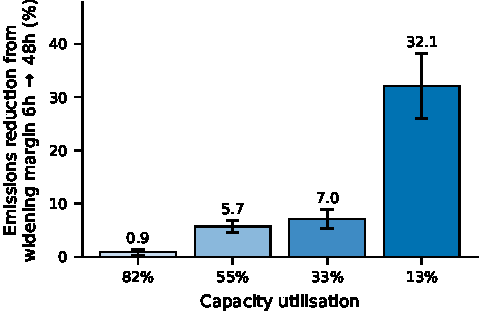
\includegraphics{figures/fig_margin_by_utilisation.pdf}
\caption{The value of deadline flexibility is conditional on load. Bars show the
reduction in attributed emissions obtained by widening the deadline margin from
6\,h to 48\,h under space+time scheduling; error bars are one standard deviation
across five workload samples.}
\label{fig:margin}
\end{figure}

\begin{table}[t]
\centering
\caption{Reduction in attributed emissions obtained by widening the deadline
margin from 6\,h to 48\,h, by capacity utilisation. Mean and standard deviation
across five workload samples.}
\label{tab:marginbyutil}
\begin{tabular}{lr}
\toprule
Capacity utilisation & Reduction from 6\,h to 48\,h margin \\
\midrule
82\,\% & \phantom{0}0.9\,\% $\pm$ 0.6 \\
55\,\% & \phantom{0}5.7\,\% $\pm$ 1.2 \\
33\,\% & \phantom{0}7.0\,\% $\pm$ 1.8 \\
13\,\% & 32.1\,\% $\pm$ 6.1 \\
\bottomrule
\end{tabular}
\end{table}

At 82\,\% utilisation the effect of deadline margin is 1.5 standard deviations
from zero and is not distinguishable from no effect at any conventional
threshold. The interpretation is mechanical rather than statistical: deferring a
request is only useful if a cleaner slot is free when the request is ready to
move, and under heavy load the cleaner slots are already occupied. Flexibility
that cannot be exercised has no value.

The saturated row of Table~\ref{tab:capmargin} carries a second qualification.
At 56 slots, between 152 and 408 of the 1\,000 requests miss their deadlines
depending on policy and margin, whereas at 84 slots and above no request does.
Emissions comparisons in the saturated regime therefore compare schedules that
are all failing, and we report that row as a boundary condition rather than as
an operating point.

\subsection{Time shifting is dominated by the choice of origin region}
\label{sec:res-home}

WaitAwhile~\cite{wiesner2021letswait} defers requests within a fixed origin region. Its reported
performance therefore depends on which region that is. We instantiate the
policy once per region of the set and examine what predicts the outcome.

Across all four capacity and margin combinations, the correlation between the
mean carbon intensity of the origin region and the emissions the policy achieves
is between $+0.941$ and $+0.998$, with a standard deviation across workload
samples of at most $0.017$. The correlation between the origin region's diurnal
amplitude and the same emissions is between $-0.066$ and $+0.085$, in every case
within one standard deviation of zero. Table~\ref{tab:homecorr} reports both.

\begin{table}[t]
\centering
\caption{What predicts WaitAwhile's emissions. Pearson correlation between the
policy's attributed emissions and two properties of its origin region, across
the seven regions of the US set. Mean and standard deviation over five workload
samples.}
\label{tab:homecorr}
\begin{tabular}{llrr}
\toprule
Capacity & Margin (h) & Origin mean CI & Origin diurnal amplitude \\
\midrule
 84 &  6 & $+0.953 \pm 0.017$ & $-0.066 \pm 0.067$ \\
 84 & 48 & $+0.941 \pm 0.016$ & $-0.007 \pm 0.076$ \\
350 &  6 & $+0.989 \pm 0.006$ & $+0.056 \pm 0.026$ \\
350 & 48 & $+0.998 \pm 0.002$ & $+0.085 \pm 0.020$ \\
\bottomrule
\end{tabular}
\end{table}

The policy's outcome is thus determined by how clean its origin grid is and not
by how much daily variation that grid offers, even though daily variation is
the only quantity the policy acts upon. The US set contains a region, CISO,
whose diurnal amplitude of 52.7\,\% is more than six times that of the flattest
region in the set; instantiating WaitAwhile there yields no advantage over
instantiating it in a region of comparable mean intensity and a quarter of the
amplitude.

The practical consequence is the spread in Table~\ref{tab:homespread}. At the
lowest utilisation, the best origin region yields 467\,kgCO\textsubscript{2}eq
and the worst 1705, a factor of 3.6. Space shifting, which is free to choose its
region per request, yields 701. The best available origin outperforms space
shifting; the median origin is worse than it by a factor of two.

\begin{figure*}[t]
\centering
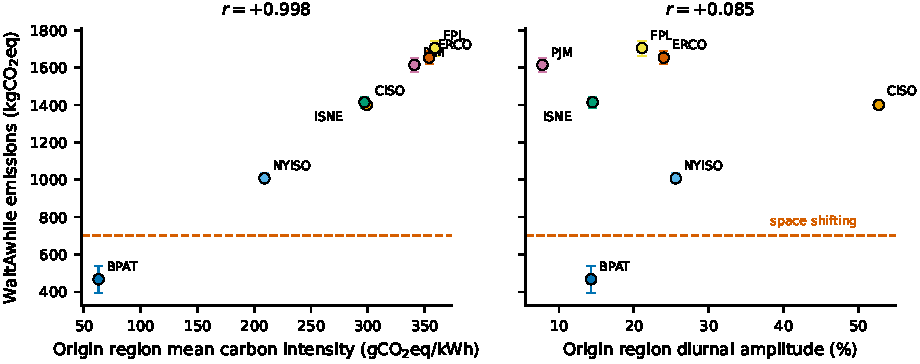
\includegraphics{figures/fig_home_region.pdf}
\caption{WaitAwhile emissions against two properties of the origin region, at
350 slots and a 48\,h margin. Each point is one of the seven candidate origins,
averaged over five workload samples; error bars are one standard deviation. The
dashed line marks space shifting in the same cell. The policy's outcome tracks
the origin's mean carbon intensity (left) and not its diurnal amplitude (right),
although the latter is the only quantity the policy acts upon.}
\label{fig:home}
\end{figure*}

\begin{table}[t]
\centering
\caption{WaitAwhile attributed emissions (kgCO\textsubscript{2}eq) across the
seven possible origin regions, with space shifting for comparison. Values are
means over five workload samples.}
\label{tab:homespread}
\begin{tabular}{llrrrr}
\toprule
Capacity & Margin (h) & Best origin & Median origin & Worst origin & Space \\
\midrule
 84 &  6 & 1841 & 1974 & 2039 & 1857 \\
 84 & 48 & 1781 & 1905 & 1984 & 1857 \\
350 &  6 &  683 & 1432 & 1698 &  701 \\
350 & 48 &  467 & 1415 & 1705 &  701 \\
\bottomrule
\end{tabular}
\end{table}

A single reported figure for a time-shifting policy is therefore a draw from a
distribution whose width exceeds the difference between the policies being
compared, and the draw is determined by a parameter that evaluations do not
customarily state. Prior work on the limits of temporal shifting
\cite{sukprasert2024limitations} does not isolate this parameter. In both region sets examined here, the conventional choice of
the first region in the candidate list happens to select the cleanest grid
available, which assigns the policy the most favourable draw.

\subsection{Reported savings scale with the composition of the region set}
\label{sec:res-regionset}

The same workload and the same scheduler were run over two region sets at
matched capacity utilisation. Table~\ref{tab:regionset} reports the reduction
that space shifting achieves relative to the carbon-agnostic baseline in each.

\begin{figure}[t]
\centering
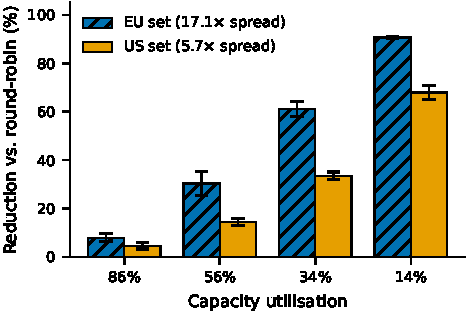
\includegraphics{figures/fig_region_set.pdf}
\caption{Reported savings scale with the composition of the candidate region
set. Identical workload, scheduler and hardware; the sets differ only in the
ratio between their cleanest region and the next cleanest. Error bars are one
standard deviation across workload samples.}
\label{fig:regionset}
\end{figure}

\begin{table}[t]
\centering
\caption{Reduction in attributed emissions from space shifting relative to
round-robin placement, at matched capacity utilisation, for two region sets.
Mean and standard deviation across workload samples (five for US, three for EU).}
\label{tab:regionset}
\begin{tabular}{lrr}
\toprule
Capacity utilisation & EU set & US set \\
\midrule
86\,\% & \phantom{0}7.8\,\% $\pm$ 1.6 & \phantom{0}4.6\,\% $\pm$ 1.4 \\
56\,\% & 30.3\,\% $\pm$ 4.9 & 14.3\,\% $\pm$ 1.5 \\
34\,\% & 61.1\,\% $\pm$ 3.2 & 33.4\,\% $\pm$ 1.6 \\
14\,\% & 90.7\,\% $\pm$ 0.4 & 67.9\,\% $\pm$ 3.0 \\
\bottomrule
\end{tabular}
\end{table}

The EU set reports roughly twice the reduction of the US set at every operating
point, and the difference exceeds the combined standard deviations in all four
rows. Nothing about the scheduler, the workload or the amount of hardware
differs between the two columns. The difference is the composition of the
candidate set: the EU set contains a region 4.7 times cleaner than its nearest
rival, so that a single destination is optimal for almost every request, whereas
in the US set the corresponding ratio is 3.3 and the placement decision remains
contested.

Regional concentration confirms the mechanism, and
Figure~\ref{fig:concentration} shows it directly. Across all valid cells of both
sets, the correlation between the share of the workload placed in the busiest
region and attributed emissions is $-0.930$ for the US set and $-0.963$ for the
EU set. In the EU set at the lowest utilisation, space shifting places 98\,\% of
the workload in a single region; in the US set it places 96\,\%. The reductions
these policies report are, to a first approximation, a measure of how much of
the workload the capacity constraint permits them to move into the cleanest
available grid.

\begin{figure}[t]
\centering
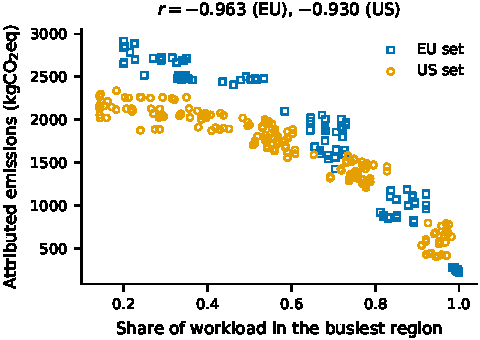
\includegraphics{figures/fig_concentration.pdf}
\caption{The mechanism common to all three findings. Each point is one
experimental cell. Emissions fall as a larger share of the workload is placed in
the busiest region, and the relationship holds across both region sets and every
capacity, deadline margin and policy examined.}
\label{fig:concentration}
\end{figure}

\subsection{Robustness}
\label{sec:res-robustness}

\paragraph{Season.} Repeating the sweep on a 720\,h window beginning in July
rather than January changes the correlation between origin carbon intensity and
WaitAwhile's emissions from the range $[+0.941, +0.998]$ to $[+0.760, +0.892]$,
and the correlation with diurnal amplitude from approximately zero to the range
$[-0.518, -0.285]$. Diurnal structure therefore acquires a secondary influence
in summer, when solar generation widens the daily cycle in several regions,
without displacing origin cleanliness as the dominant term. The ordering of
policies is unchanged.

\paragraph{Workload class.} Restricting the workload to the class the provider
labels delay-insensitive preserves the result, with the correlation between
origin carbon intensity and emissions at $+0.822$, $+0.920$ and $+0.936$ in
three of four cells. The exception is the combination of tight capacity and wide
margin, where the correlation with origin intensity falls to $+0.403$ and that
with diurnal amplitude rises to $+0.776$: when capacity constrains relocation
and the deadline permits deferral, temporal structure is the only remaining
lever and briefly becomes the dominant one.

This class also differs from the general mixture in a way that bears on the
premise of deadline-based scheduling. Its mean virtual machine lifetime is
340.7\,h against 34\,h for the unrestricted sample, an order of magnitude
longer. A 48\,h margin therefore represents 141\,\% of the mean lifetime in the
general mixture but only 14\,\% in the class explicitly designated as tolerant
of delay. The population with the most permission to wait has the least relative
room in which to do so.

\paragraph{Power model.} Repeating the entire sweep under the linear 120/480\,W
model in place of the measured curve raises absolute emissions by approximately
40\,\% but leaves every reported proportion within its sampling spread: the
capacity effect moves from 77.4\,\% $\pm$ 2.3 to 75.9\,\% $\pm$ 2.2, the margin
effect at 82\,\% utilisation from 0.9\,\% $\pm$ 0.6 to 1.0\,\% $\pm$ 0.5, the
correlation with origin intensity from $[+0.941, +0.998]$ to
$[+0.943, +0.998]$, and the EU-to-US ratio at the lowest utilisation from
90.7/67.9 to 90.1/67.1. The conclusions of
Sections~\ref{sec:res-capacity}--\ref{sec:res-regionset} are therefore not
artefacts of the power model adopted.

The absolute values are not invariant, and the direction of the change is worth
recording. Under the measured curve, round-robin placement rises by 44\,\%
while the carbon-aware policies rise by 26\,\% or less, so the reduction
attributed to space shifting increases rather than decreases. The attributed
basis charges the full draw of every host carrying load, and the measured
machine idles at 55\,\% of peak rather than 25\,\%; raising the fixed cost of
activating a host penalises the policy that activates the most. Round-robin
placement leaves 72 hosts active at the lowest utilisation against 47 for space
shifting and 38 for space+time. Part of what the attributed basis records as a
carbon-aware saving is therefore a consolidation saving. The dynamic basis,
which excludes idle draw entirely, separates the two: on that basis the same
comparison yields reductions of 64\,\% and 71\,\% respectively, confirming that
regional placement rather than consolidation accounts for the larger share.

\section{Discussion}
\label{sec:discussion}

\subsection{What these results imply for reporting}

The three parameters examined here are not exotic. Each is fixed in the course
of designing any evaluation of carbon-aware scheduling, and each is ordinarily
left unstated. Their combined effect, in our experiments, spans reported
reductions from 4.6\,\% to 90.7\,\% for the same class of policy. A figure
reported without them is therefore not comparable with a figure reported
elsewhere, and the divergence in the literature is to that extent expected
rather than anomalous.

Four items would make such figures comparable.

\emph{Capacity utilisation.} Total demand as a fraction of total available
slot-hours, stated alongside any claim about deadline flexibility. Without it, a
reduction attributed to flexibility cannot be distinguished from a reduction
attributable to an unconstrained pool.

\emph{Origin region.} For any policy that shifts in time but not in space, the
region in which the workload originates, and preferably the distribution of
results across candidate origins rather than a single value.

\emph{Region-set composition.} The candidate regions and their mean carbon
intensities, from which a reader can judge whether the set admits a dominant
optimum. The ratio between the cleanest region and the second cleanest is a
compact summary.

\emph{Accounting basis.} Whether reported emissions include the idle draw of
provisioned hosts, of active hosts only, or neither. As
Section~\ref{sec:accounting} shows, the first of these cannot distinguish
policies at all in a fixed-fleet setting, and the second conflates regional
placement with consolidation.

\subsection{Concentration and deployability}

The mechanism common to all three findings is concentration. Across every valid
cell in both region sets, the correlation between the share of work placed in
the busiest region and attributed emissions is below $-0.93$. The policies
reduce emissions by moving work into the cleanest reachable grid, and the three
parameters govern how much of the workload can be moved, where a constrained
policy starts from, and how much is gained by arriving.

This has an uncomfortable consequence. The configurations that report the
largest reductions are those in which 95\,\% or more of the workload is placed
in one region, and that is not a configuration any operator could adopt. Real
deployments are constrained by data residency, by latency to users, by capacity
that is finite in exactly the way our capped configurations model, and by the
grid-level effects of concentrating demand. The reductions reported at low
utilisation should therefore be read as upper bounds obtained under a placement
distribution that would not survive contact with those constraints, rather than
as achievable savings.

Read the other way, the result is more encouraging than it first appears. The
82\,\% utilisation row, where deadline flexibility is worth 0.9\,\% and space
shifting 4.6\,\%, is the row that most resembles an efficiently operated
facility. That the returns are small there is a finding about where effort is
best directed, not an argument against carbon-aware scheduling as such.

\subsection{On the interpretation of time shifting}

Section~\ref{sec:res-home} shows that a time-shifting policy's outcome tracks
the mean intensity of its origin rather than that origin's temporal structure.
The natural reading is that temporal flexibility is worth little. The more
precise reading is that temporal flexibility is worth little \emph{when spatial
flexibility is available and capacity is not binding}, which is the regime in
which the two are usually compared. Our delay-insensitive robustness condition
supplies the counterexample: at tight capacity and wide margin, where
relocation is constrained and deferral is not, the correlation with origin
intensity falls to $+0.403$ and that with diurnal amplitude rises to $+0.776$.
Temporal structure becomes the dominant term exactly when it is the only term
available.

A second observation from that condition bears on the premise of deadline-based
scheduling. The workload class the provider designates as delay-insensitive has
a mean lifetime an order of magnitude longer than the general mixture, so that a
given absolute margin represents a far smaller fraction of runtime. Deadline
margins expressed in hours are not comparable across workload classes, and
margins expressed as a fraction of runtime would be a more meaningful axis for
future studies.

\section{Limitations}
\label{sec:limitations}

\emph{Perfect foresight.} Planning is performed against the ground-truth carbon
trace. This isolates the parameters under study from prediction error, but it
means the absolute reductions reported here are upper bounds with respect to
forecast quality. Whether the three effects survive realistic forecast error is
a question we address separately.

\emph{Single workload source.} All virtual machine requests derive from one
provider's 2019 trace. The duration and size distributions of that trace shape
the capacity utilisations at which our effects appear, and a workload with a
different shape would place the transition points elsewhere, though we have no
reason to expect the direction of the effects to change.

\emph{Deadline margins are imposed rather than observed.} The trace records a
workload category but not a service-level objective, so deadline margins are
assigned as an experimental factor rather than read from the data. The
delay-insensitive condition is the closest available approximation to a
provider-designated flexibility class.

\emph{No migration or preemption.} Virtual machines run to completion where they
start, following the formulation of the work we build on. Policies permitting
mid-flight migration would have a larger action space, and the capacity
interaction we report might take a different form under them.

\emph{Excluded costs.} Network transfer between regions, the embodied carbon of
the hardware, and datacentre overhead beyond the host itself are not modelled.
The first of these is of particular relevance given that the largest reductions
we observe coincide with the greatest concentration of load.

\emph{Two region sets.} The claim of Section~\ref{sec:res-regionset} rests on a
contrast between two sets. The direction of the effect follows from the
mechanism and we expect it to generalise, but the coefficient relating
region-set composition to reported savings is not established by two points.


% ---------------------------------------------------------------
\section{Conclusion}
\label{sec:conclusion}

The reductions reported for carbon-aware virtual machine scheduling depend on
three parameters that evaluations do not customarily state. Capacity
utilisation determines whether deadline flexibility has any value at all,
varying its worth from 32\,\% to under 1\,\% across the range we examine. The
origin region assigned to a time-shifting policy determines that policy's result
more completely than the temporal structure it is designed to exploit, with a
spread across candidate origins of a factor of 3.6. The composition of the
candidate region set determines how much a spatial policy can gain, with one set
reporting twice the reduction of another under identical conditions. All three
operate through the same mechanism, the concentration of work into the cleanest
reachable grid, and the configurations that report the largest reductions are
those in which nearly the entire workload is placed in a single region. We
recommend that capacity utilisation, origin region, region-set composition and
carbon accounting basis be reported alongside any figure for carbon-aware
scheduling, and we note that the returns are smallest in precisely the
high-utilisation regime that an efficiently operated facility occupies.

% ---------------------------------------------------------------
\section*{Declaration of competing interest}

The authors declare that they have no known competing financial interests or
personal relationships that could have appeared to influence the work reported
in this paper.

\section*{Data availability}

The carbon intensity traces are published by the CarbonCast project and the
virtual machine traces by the Azure Public Dataset; both are cited in the text.
The simulation code, the trace preparation and analysis scripts, and the result
files underlying every figure and table in this paper are available at
REPOSITORY URL.

\section*{Acknowledgements}

FUNDING AND ACKNOWLEDGEMENTS.

% ---------------------------------------------------------------
\bibliographystyle{elsarticle-num}
\bibliography{refs}

\end{document}
